\chapter{Технологический раздел}

В данном разделе описывается реализация разработанной системы и демонстрационной программы, средстава разработки, сборки и развертывания, а также тестирование.

\section{Выбор средств программной реализации}

Так как целью работы является разработка библиотеки для языка Haskell, целесообразно вести разработку на этом же языке. Язык Haskell относится к функциональным языкам общего назначения и обладает следующими особенностями:

\begin{itemize}
\item Чистые функции. Большинство функций в языке Haskell являются чистыми, то есть детерминированными и не имеющими побочных эффектов. При использовании таких функций программист может быть уверен, что при вызове такой функции не будет произведено каких-либо неявных действий (запись даных в файл, изменение значения переданных параметров, изменеие состояния некоторого объекта и т.п.) и на одних и тех же входны параметрах функкция всегда вернет одинаковый результат. Это существенно упрощает разраотку и тестирование программ.

\item Ленивые вычисления. Все вычисления в Haskell по умолчанию являются ленивыми, то есть ни одно значение не будет вычислено до тех пор, пока его значение действительно не понадобится. Этот механизм позволяет экономить выислительные мощности и работать со структурами вроде бесконечных списков. Однако при неаккураьном использовании это может привести к неэффективному расходованию памяти.

\item Строгая статическая типизация. Строгая типизация позволяет писать более надежные программы, так как несоответствие типов приведет к сообщению об ошибке, а не к некорректному поведению программы и будет быстрее обнаружено и исправлено. Статическая типизация позволяет выявить такие ошибки еще на этапе компиляции программы.

\item Автоматическое управление памятью. Как и большинство современных языков программирования Haskell берет на себя выделение и освобождение памяти. Это гарантировать отсутствие в разрабатываемой программе таких ошибок как переполнение буфера, неинициализированные переменные и т.п.

\end{itemize}

Помимо этого для Haskell существует обширный централизованный архив библиотек Hackage\cite{hackage}, и поисковая система Hoogl\cite{hoogle}, позволяющая найти описание функции не ттолько по ее названи но и по сигнатуре.

\subsection{Построение графиков}

Для построения графиков была выбрана система Gnuplot\cite{gnuplot}. Это свободно распространяемая, кросплатформенная программа предназначенная для построения двух- и трехмерных графиков функций, заданных как аналитически, так и в виде наборов данных. Gnuplot поддержвает вывод результатов в различных форматах: растровых (PNG, JPEG), векторных (SVG, PDF), в виде кода LaTeX, в интерактивном режиме и др. Система используется для построения графиков в таких математических пакетах как GNU Octave, Maxima и других.

Для использования возможностей Gnuplot в программах на Haskell существует несколько библиотек, опубликованных на Hackage. В данной работе была использована библиотека EasyPlot.


\subsection{Построение пользовательского интерфейса}

Для построения пользовательского интерфейса демонстрационной программы была использована библиотека wxHaskell\cite{wxhaskell}, которая в свою очередь является оберткой вокруг библиотеки для построения пользовательского интерфейса на C++ wxWidgets. 

Особенности wxWidgets:

\begin{itemize}
\item Созданные с помощью данной библиотеки приложения переносимы на большинство современных ОС.

\item В разработанном интерфейсе используются элементы управления привычные для пользователей целевой ОС. То есть стиль интерфейса программы будет отличаться на различных ОС и будет соответствовать рекомендуемому стилю для конкретной системы.

\end{itemize}

wxHaskell является надстройкой над wxWidgets, позволяющей создавать графический интерфейс к программам на языке Haskell. Она поддерживает большую часть функционала wxWidgets, позволяет описывать интерфейс в <<декларативном>> стиле с использованием функциональных связок и абстракцй высокого уровня. Библиотека особенно удобна для создания демонстрационных версий программ, так как во многом берет на себя решение адачи корректного расположения элементов управления на экране. 

\subsection{Сборка и развертывание библиотеки}

Для сборки разработанной библиотеки и развертывания ее на целевой машине была использована система Cabal. Данная система предоставляет единый интерфейс для создания и установки инсталяционных пакетов с программами и библиотеками на Haskell. Система связана с архивом библиотек Hackage и позволяет устанавливать хранящиеся там пакеты и оформить собственную программу в виде пакета для Hackage.

Информация о создаваемом пакете указывается в файле \Code{.cabal} в директории проекта. В нем указываются:
    
\begin{itemize}
\item имя пакета;

\item текущая версия;

\item информация об авторе и лицензии;

\item допустимые версии компилятора;

\item используемые расширения компилятора;

\item входящие в состав пакета библиотеки и исполняемые программы;

\item пакеты Hackage, необходимые для работы пакета;

\item и др.

\end{itemize}
    
    
Фрагмент файла \Code{.cabal} для разработаной библиотеки приведен ниже.

\lstinputlisting[caption=Фрагмент описания пакета,label=lst:cabal]{inc/src/.cabal}

Сборка и установка пакета выполняется следующими командами:

\begin{itemize}
\item \Code{cabal configure}~--- подготовка к сборке программы: определение целевой платформы, зависимостей и др.;

\item \Code{cabal build}~--- запуск процесса компиляции;

\item \Code{cabal install}~--- установка пакета в систему. Включает в себя первые две комманды;

\item \Code{cabal clean}~--- удаляет все временные файлы созданные предыдущими коммандами;

\end{itemize}
    
    

%\section{Демонстрационная программа}

%Для демонстрации возможностей разработанной библиотеки, а также в целях дополнительного тестирования была разработанна демонстрационная программа. В программе производится расчет производительности системы массового обслуживания при заданных параметрах и варьировании одного из них. Расчет производительности ведется как путем имитационного моделирования при помощи разработанной бибилиотеки, так и с помощью аналитической модели. Программа выводит на экран графики, позвооляющие сравнить значения полученные путем моделирования с полученными теоретически. Структура разработанной программы показа на рисунке~\ref{fig:demoStruct}



\section{Тестирование}

Для модульного тестирования разработанной библиотеки использовалась библиотека HUnit\cite{HUnit}. Это фреймворк основанный на идеях JUnit, но предназначенный для тестированя программ на Haskell.

Типичный базовый тест состоит из текстового описания, вычисляемого выражения и ожидаемого результата. Базовые тесты объединяются в группы, те, в свою очередь, могут объединяться в большие группы и т.д. В итоге образуется единая древовидная структура тестов. Ниже показан пример описания теста.

\begin{verbatim}
emptyFEC = TestCase (assertEqual "for (addFE [] (1,defTransact))," 
                                 ([(1,defTransact)]) 
                                 (addFE [] (1,defTransact))
                    )
\end{verbatim}

По результатам выполнения тестов HUnit выводит следующую статистику: общее число тестов, число проведенных тестов, число тестов вызвавших непредвиденное исключение (что говорит об ошибке в самом тесте) и число тестов, закончившихся неудачей (что обычно говорит об ошибке в тестируемой программе).

В таблице~\ref{tab:chainsTest} приведен протокол тестирования функции \Code{addFE}, добавляющей новое событие в список будущих событий.


\begin{table}[h!]
\caption{}
\label{tab:chainsTest}
\begin{tabular}{|l|p{0.7\textwidth}|}
\hline
Название теста & emptyFEC\\
\hline
Описание теста & Добавление события в пустой список\\
\hline
Ожидаемый результат & Список из одного события\\
\hline
Результат & Тест пройден\\
\hline
\hline
Название теста & nearestAddFE\\
\hline
Описание теста & Добавление в список события с наименьшим временем наступления\\
\hline
Ожидаемый результат & Добавленное событие становится первым в списке\\
\hline
Результат & Тест пройден\\
\hline
\hline
Название теста & lastAddFE\\
\hline
Описание теста & Добвление в списко события с наибольшим временем наступления\\
\hline
Ожидаемый результат & Добавленное событие становится последним в списке\\
\hline
Результат & Тест пройден\\
\hline
\hline
Название теста & middleAddFE\\
\hline
Описание теста & Добавление в список события с промежуточным временем наступления\\
\hline
Ожидаемый результат & Добавленное событие занимает место в списке в соответствии со своим временем наступления\\
\hline
Результат & Тест пройден\\
\hline
\hline
Название теста & multyAddFE\\
\hline
Описание теста & Добавление в список события с тем же  временем наступления, что и у  одного из событий в списке\\
\hline
Ожидаемый результат & Добавленное событие занимает место в списке сразу за событием с тем же временем наступления\\
\hline
Результат & Тест пройден \\
\hline
\end{tabular}
\end{table}

В общей сложности было проведено 84 теста. Вывод тестовой программы представлен ниже.

\begin{verbatim}
Cases: 84  Tried: 84  Errors: 0  Failures: 0
\end{verbatim}


\subsection{Тестирование стохастических функций}

При организации имитационного моделирования важную роль играют функции генерации случайных величин с заданным законом распределения. При тестировании таких функций приходится отказаться от описанного выше принципа <<выражение --- ожидаемое значение>>, поскольку результат вычисления функции различается от запуска к запуску.

Для тестирования таких функций следует многократно вычислить значение тестируемой функции и сравнить собранную статистику с ожидаемым распределением. В даннной работе в качестве критерия соответствия полученных значений ожидаемому распределению использовался критерий согласия Пирсона.

Для вычисления статистики по этому критерию и вычисления квантилей распределения $\chi^2$ и спользовался пакет statistics из архива библиотек Hackage.

\subsection{Сравнение аналитической и имитационной модели}

В качестве дополнительной проверки на корректность разработанных алгоритмов и безошибочность их реалиации был проведен ряд опытов с демонстрационной программой. Были построены графики зависимости производительности моделируемой системы от различных параметров при прочих фиксированных параметрах.

\subsection*{Опыт 1}

Варьируется число задач в системе. Количество процессоров и каналов равно единицы. Интенсивность обдумывания равна единице. Отказов и восстановлений нет. Интенсивности обработки на канальной и процессорной фазе равны 5. Результаты показаны на рисунке~\ref{fig:plot1}.

\begin{figure}[ht]
  \centering
  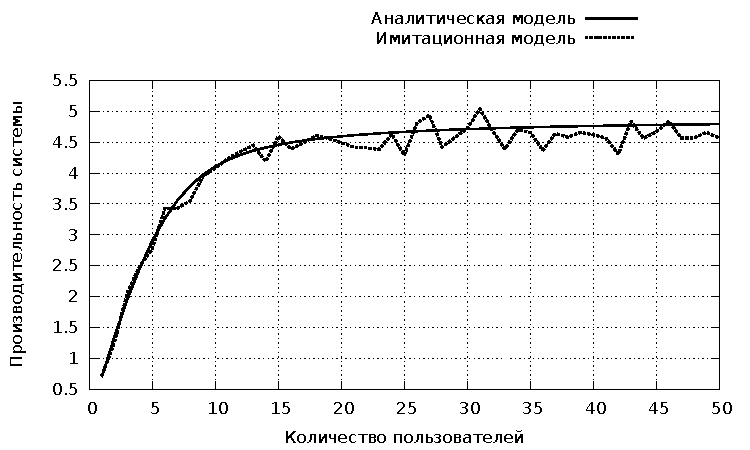
\includegraphics[width=\textwidth]{inc/pdf/plot1}
  \caption{Опыт 1}
  \label{fig:plot1}
\end{figure}

\subsection*{Опыт2}

Опыт проводится при тех же параметрах, но число каналов и интенсивность обслуживания на процессороной фаззе увеличены в двое. Результаты показаны на~\ref{fig:plot1a}.

\begin{figure}[ht]
  \centering
  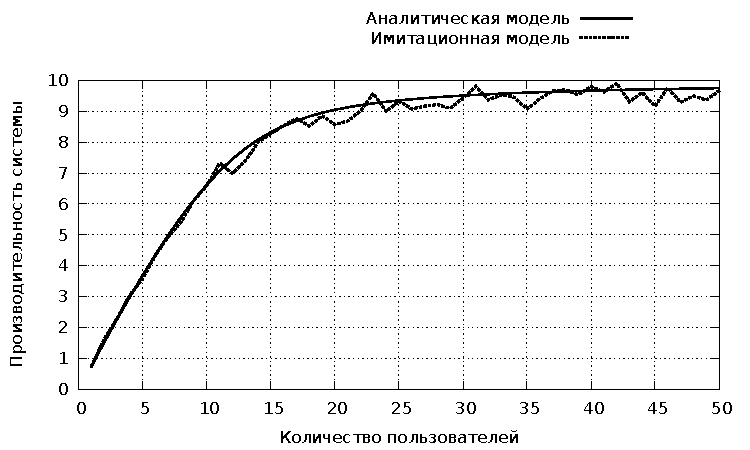
\includegraphics[width=\textwidth]{inc/pdf/plot1a}
  \caption{Опыт 2}
  \label{fig:plot1a}
\end{figure}


\subsection*{Опыт3}

Варьируется число процессоров. Число задач и каналов равняется 10. Итенсивность обдумывания равна единице. Интенсивности обработки задач на процессороной и канальной фазах равны 5. Результаты опыта показаны на рисунке~\ref{fig:plot2}.

\begin{figure}[ht!]
  \centering
  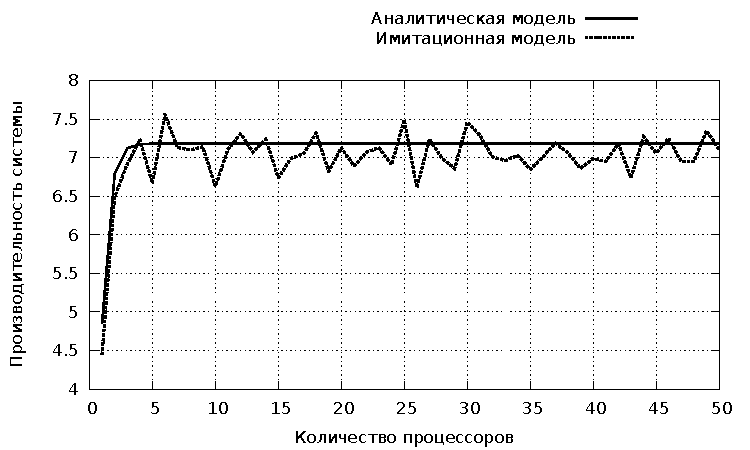
\includegraphics[width=\textwidth]{inc/pdf/plot2}
  \caption{Опыт 3}
  \label{fig:plot2}
\end{figure}

\subsection*{Опыт4}

Опыт проводится при тех же параметрах, что и предыдущий, но количество каналов уменьшено вдвое. Результаты опыта показаны на рисунке~\ref{fig:plot2a}.

\begin{figure}[ht!]
  \centering
  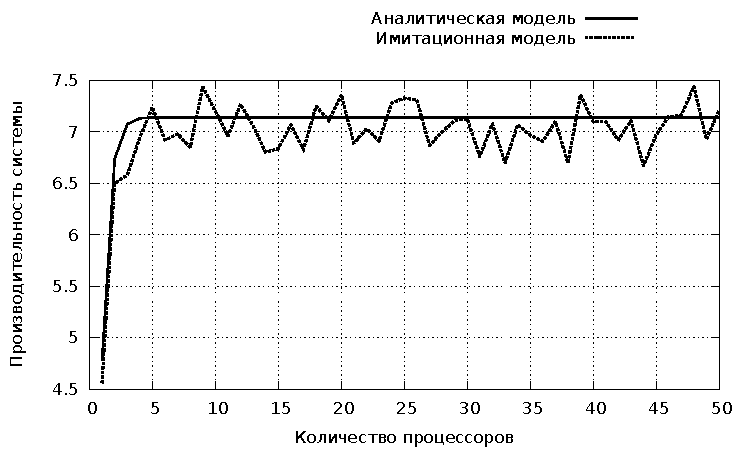
\includegraphics[width=\textwidth]{inc/pdf/plot2a}
  \caption{Опыт 4}
  \label{fig:plot2a}
\end{figure}

\subsection*{Опыт5}

Варьируется интенсивность обработки на канальной фазе. количество задач равно 10. Количество процессоров и каналов равно 4. Интенсивность обдумывания~--- 5, интенсивность обработки на процессорной фазе~--- 20 Результаты опыта показаны на рисунке~\ref{fig:plot3}.

\begin{figure}[ht!]
  \centering
  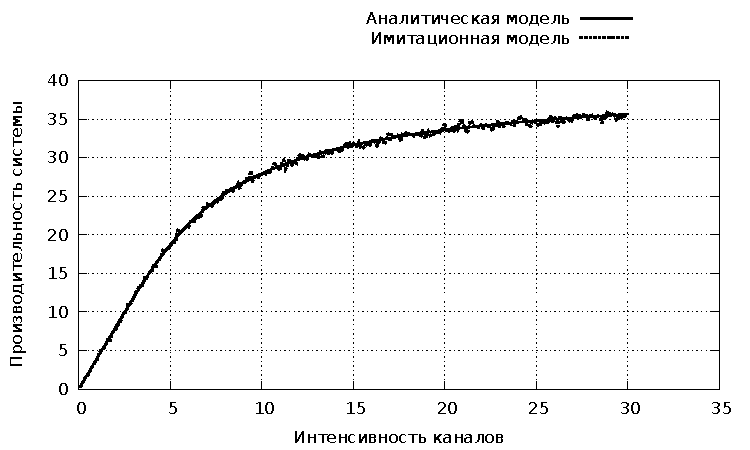
\includegraphics[width=\textwidth]{inc/pdf/plot3}
  \caption{Опыт 5}
  \label{fig:plot3}
\end{figure}

\subsection*{Опыт6}

Опыт проводится при тех же параметрах, что и предыдущий, но количество задач уменьшено вдвое. Результаты опыта показаны на рисунке~\ref{fig:plot3a}.

\begin{figure}[ht!]
  \centering
  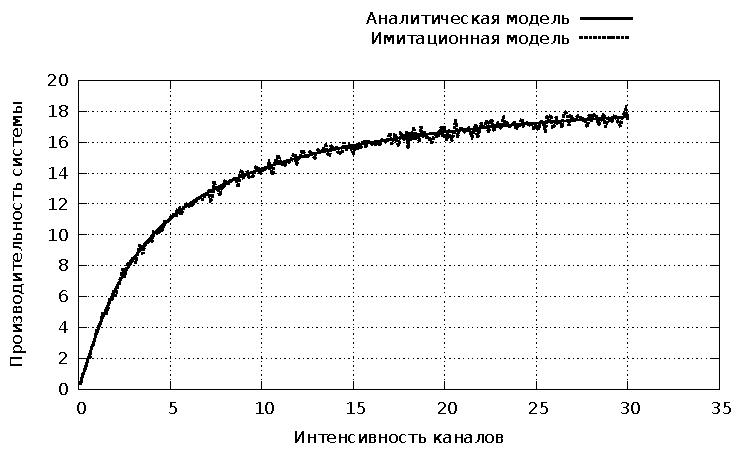
\includegraphics[width=\textwidth]{inc/pdf/plot3a}
  \caption{Опыт 6}
  \label{fig:plot3a}
\end{figure}

\subsection*{Опыт7}

Варьируется интенсивность отказов процессоров. Количество задач равно 10. Количество процессоров и каналов равно 4. Интенсивность обдумывания~--- 1, интенсивность обработки на процессорной  и канальной фазах~--- 3. Интенсивность восстановления процессоров равна 10. Количество ремонтных бригад~--- 5.Результаты опыта показаны на рисунке~\ref{fig:plot4}.


\begin{figure}[ht!]
  \centering
  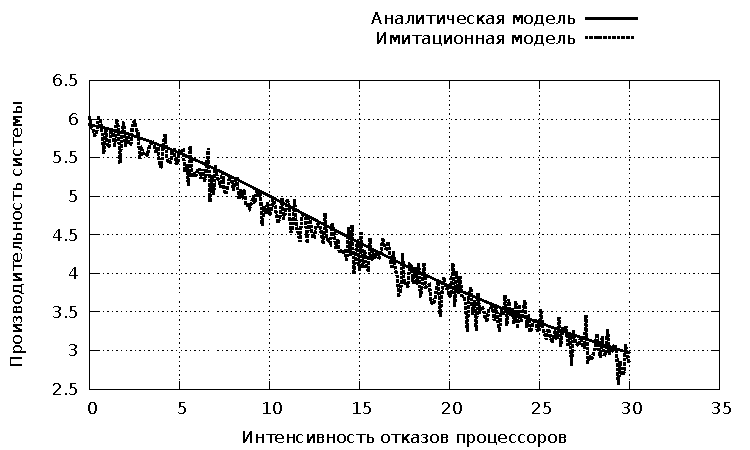
\includegraphics[width=\textwidth]{inc/pdf/plot4}
  \caption{Опыт 7}
  \label{fig:plot4}
\end{figure}

\subsection*{Опыт8}

Опыт проводится при тех же параметрах, что и предыдущий, но интенсивность восстановления процесоров уменьшена вдвое. Результаты опыта показаны на рисунке~\ref{fig:plot4a}.

\begin{figure}[ht!]
  \centering
  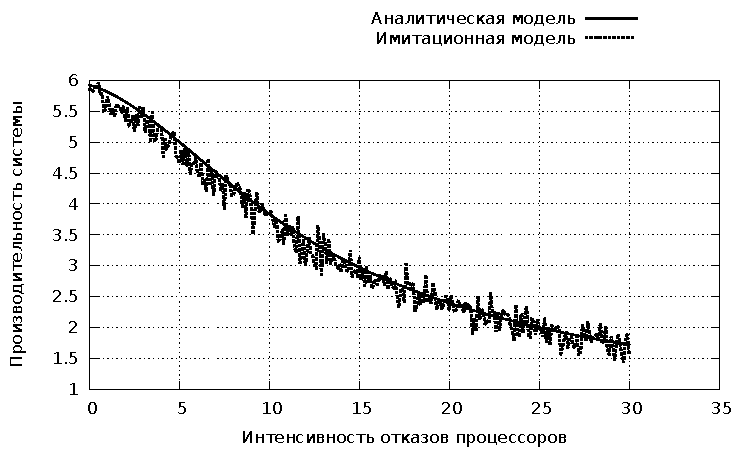
\includegraphics[width=\textwidth]{inc/pdf/plot4a}
  \caption{Опыт 8}
  \label{fig:plot4a}
\end{figure}

\subsection*{Опыт9}

Варьируется количество ремонтных бригад. Количество задач и процессоров~--- 5. Количество кканалов 15. Интенсивность обдумывания~---1. Интенсивность обработки на процессорной и канальной фазах~---5. Интенсивность отказов каналов~---14, интенсивность восстановлений~---7. Результаты опыта показаны на рисунке~\ref{fig:plot5}.

\begin{figure}[ht!]
  \centering
  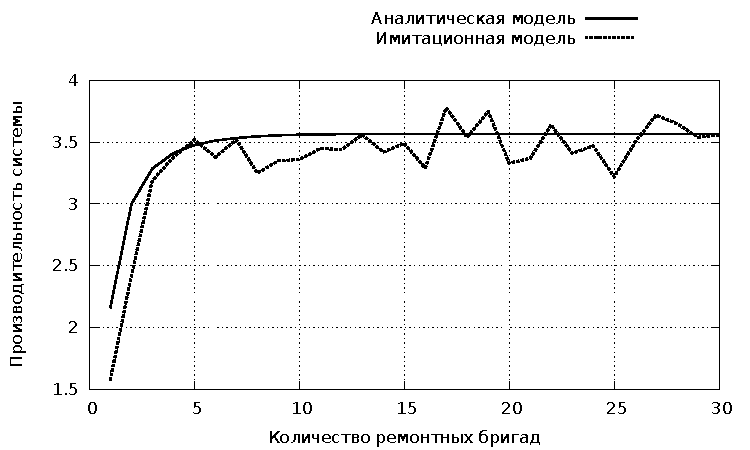
\includegraphics[width=\textwidth]{inc/pdf/plot5}
  \caption{Опыт 9}
  \label{fig:plot5}
\end{figure}

\subsection*{Опыт10}

Опыт проводится при тех же параметрах, что и предыдущий, но интенсивность восстановления взята равной интенсивности отказов. Результаты опыта показаны на рисунке~\ref{fig:plot5a}.

\begin{figure}[ht!]
  \centering
  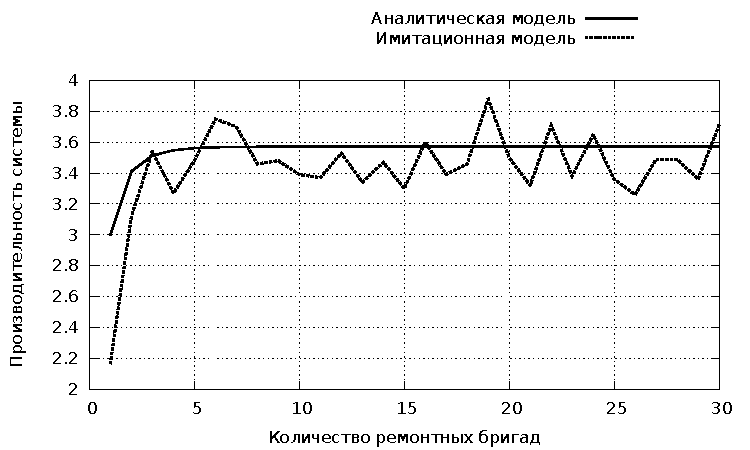
\includegraphics[width=\textwidth]{inc/pdf/plot5a}
  \caption{Опыт 10}
  \label{fig:plot5a}
\end{figure}

Из проведенных опытов видно, что данные полученные при помощи разработанной библиотеки и имитационной модели качественно соответствуют результатам анаолитических исследований. Некоторый разброс значений объясняется стохастическим характером модели.

\section{Выводы}

Были реализованы разработанные в предыдущем разделе методы и алгоритмы. Разработанная бибилиотека была протестирована при помощи модульного тестирования. Также был проведен ряд опытов подтверждащих адекватность построенной имитационной модели и корректность реализованных алгоритмов.
